\setchapterpreamble[u]{\margintoc}¡

\chapter{Experimental Evaluation on Neural Networks}
\labch{evaluation-on-neural-networks}

\marginemptybox{7cm}

In this chapter, we investigate whether our two impact quantifiers for neural networks, \cf{} \changesname{} and \qlibraname{}, successfully quantify variations in the usage of input features. Specifically, \refsec{eval-changes} evaluates the effectiveness of \changesname{} by comparing it to two \emph{feature importance metrics}, which are commonly used to evaluate the relevance of input features in making predictions within a machine learning model. \refsec{eval-qlibra} evaluates \qlibraname{} on neural networks trained on the Adult dataset\sidenote{\label{adult-url}\rurl{archive.ics.uci.edu/ml/datasets/adult}} from the UCI Machine Learning Repository to discover the amount of fair input space. This chapter is partially based on the evaluation section of the work presented at the 28th Static Analysis Symposium (SAS) 2021~\sidecite[][Section 3]{Mazzucato2021}.

\frenchdiv

\emph{
  Dans ce chapitre, nous examinons si nos deux quantificateurs d'impact pour les réseaux neuronaux, \cf{} \changesname{} et \qlibraname{}, permettent de quantifier efficacement les variations dans l'utilisation des caractéristiques d'entrée. Plus précisément, \refsec{eval-changes} évalue l'efficacité de \changesname{} en le comparant à deux \emph{mesures d'importance des caractéristiques}, qui sont couramment utilisées pour évaluer la pertinence des caractéristiques d'entrée dans les prédictions d'un modèle d'apprentissage automatique. \refsec{eval-qlibra} évalue \qlibraname{} sur des réseaux neuronaux entraînés sur le jeu de données Adult\sidenotemark[\ref{adult-url}] de la UCI Machine Learning Repository pour découvrir la quantité d'espace d'entrée équitable. Ce chapitre est partiellement basé sur la section d'évaluation du travail présenté lors du 28e Symposium sur l'analyse statique (SAS) 2021~\cite[Section 3]{Mazzucato2021}.
}

\section{Evaluation of \changesname{}}[\changesname]
\labsec{eval-changes}



For the evaluation of \changesname, we implemented this evaluation prototype as part of the tool \impatto\sidenote{\impattourl}, \cf{} \refch{showcase}, in \python{}.
We extended the front-end of \impatto{} to handle neural networks written in \python{} format, and the backend to support the abstract analysis of neural networks, \cf{} \refsec{neural-network-abstract-analysis}. This prototype implements the \abstractchangesname{} abstract quantifier, which is used to quantify the impact of input features on the output of a neural network. All neural network models used in this evaluation are open source and part of \impatto.
In particular we instrument \impatto{} to use \abstractchangesname{} starting from the output buckets representing all the target classes in the model, one for each bucket: $\buckets = \vecdef{\{\bigwedge_{j'\le m} x_{\outputlayer, j'}\le x_{\outputlayer, j}\}}{j\le m}$.


For our evaluation, we used public datasets from the online community platform Kaggle\sidenote{\rurl{www.kaggle.com}} to train several neural network models.
We focused on four datasets: ``\wine''~\sidecite{Cortez2009}, ``\diabetes''~\sidecite{Smith1988}, ``\rain''~\sidecite{Young2019}, and ``\princess''~\sidecite{Unmoved2023}.
We pre-processed the ``\rain'' database and removed non-continuous input features, as we do not support discrete input features yet.
To preserve data consistency, since the majority of daily weather observations were collected in Canberra, we eliminated the observations from other stations.
As a result of this pre-processing step, we retained approximately 2000 entries, aligning with the sizes of other datasets.
We trained about 700 networks per database by permuting the network structure and number of input features to obtain a uniform benchmark.
The number of input features ranges from at least 3, to the number of attribute of the databases (after pre-processing),
respectively, 10 attributes for ``\wine,'' 8 for ``\diabetes'', 17 for ``\rain'', and 13 for ``\princess''.
The model size ranges from 2 to 6 hidden layers, each with 3 to 6 nodes, for a total of 6 to 36 nodes for each network model.
This relatively small network size is chosen as a proof-of-concept evaluation to study \changesname{} without the need for extensive computational resources.
All models were trained with Keras\sidenote{\rurl{github.com/keras-team/keras}}, using the Adam optimizer~\sidecite{Kingma2014} with the default learning rate, and binary crossentropy as the loss function. Each model was trained for 150 iterations.
The obtained neural network accuracy usually depends on the chosen subset of input features which is usually lower than the accuracy achieved in the literature.
However, we remark that our study focuses on the impact analysis, therefore high accuracy is not needed in our benchmarks.

% We implemented $\abstractchangesname$ in \python{}, as part of the tool \impatto\sidenote{\impattourl}.
% All models used in our experiments are open source as part of \impatto.
% In particular, we instrument \impatto{} to use $\abstractchangesname$  starting from the output buckets represent all the target classes in the model $\defmodel$, one for each bucket: $\buckets = \vecdef{\{\bigwedge_{j'\le m} x_{\outputlayer, j'}\le x_{\outputlayer, j}\}}{j\le m}$.
% For each model, we assume a uniform distribution of the input space.


To empirically check that \impatto{} specialized with $\abstractchanges$, behaves similarly to $\changesname$, we uniformly sample 1000 points in the input space of the network and then apply $\changesname$ to this set; we refer to this result as the \textit{baseline}.
This approach is not sound as we could miss changes in the outcome not exploited by unsampled points, however it is overall a close-enough approximation of $\changesname$.
%
We compare the result of \impatto{} with baseline employing four heuristics, called maximum common prefix length (\mcpl), relaxed maximum common prefix length (\rmcpl), Euclidean distance (\euclidean), and Manhattan distance (\manhattan), defined below.
% Let $\defaultanalysisletter\in\simpleset{\pfi,\rfe, \impatto}$ be an analysis, defined as a mapping from a neural network model $\defmodel$ and an input feature $\definputvariable$, to a quantity value.
% In particular,

Given two analyses $F, F'$ (\eg, \impatto{} and baseline), the heuristic (\mcpl) first sorts the result of the analyses $F, F'$ applied to all the input features, by decreasing order.
The heuristic then returns the corresponding indices of the sorted results.
Formally, it computes $I=\argsort_\definputvariable F(\defmodel, \definputvariable)$ and $J=\argsort_\definputvariable F'(\defmodel, \definputvariable)$ for the two analyses respectively, where $\argsort$ returns the corresponding indices of the sorted list (by decreasing order), \eg, $\argsort \langle 30, 65, 2, 60 \rangle = \langle 2,4,1,3\rangle$.
Afterwards, (\mcpl) retrieves the length of the maximal common prefix between $I$ and $J$:
\begin{align}\labeq{mcpl}
  \mcpl(I, J) \DefeQ
  \begin{cases}
    1+\mcpl(\langle i_2, \dots, i_m \rangle, \langle j_2, \dots, j_m \rangle) \\ \quad \text{if } I = \langle i_1, \dots, i_m \rangle \land  J = \langle i_1, \dots, j_m \rangle\\
    0 \\ \quad \text{otherwise}
  \end{cases}
\end{align}
For instance, assuming $I=\langle 4,1,2,3,5 \rangle$ and $J=\langle 4,1,2,5,3 \rangle$, $\mcpl(I, J)= 3$ since the maximum common prefix is $\langle 4,1,2\rangle$ of length 3. The relaxed variation (\rmcpl) allows a 10\% of overlap among quantity values, \eg, given $\vecdef{F(\defmodel, \definputvariable)}{\definputvariable} = \langle 0.4, 0.95, 0.6, 1 \rangle$ and $\vecdef{F'(\defmodel, \definputvariable)}{\definputvariable} = \langle 30, 65, 2, 60 \rangle$, we obtain $I=\argsort \langle 0.4, 0.95, 0.6, 1 \rangle = \langle 4, 2, 3, 1 \rangle $ and $J=\argsort \langle 30, 65, 2, 60 \rangle = \langle 2, 4, 1, 3 \rangle$, hence $\mcpl(I, J)$ would return 0. However, a 10\% of margin of error permits to swap the indices of values 0.95 and 1 in the first list obtaining $\langle 2, 4, 3, 1 \rangle$, we say that $I$ is equivalent to $\langle 2, 4, 3, 1 \rangle$ (written $I\simeq\langle 2, 4, 3, 1 \rangle$), hence $\mcpl(\langle 2, 4, 3, 1 \rangle, J)=2$. Formally,
we define \rmcpl{} as the maximum of \mcpl{} of all the possible equivalences:
\begin{align}\labeq{rmcpl}
  \rmcpl(I, J) \DefeQ \max \setdef{\mcpl(I', J')}{{I' \simeq I \land J' \simeq J}}
\end{align}
The Euclidean distance is defined as $\euclidean(I, J) \defeq \sqrt{\sum_k (I_k - J_k)^2}$, and the Manhattan distance as $\manhattan(I, J) \defeq \sum_k \cardinality{I_k - J_k}$.

\subsection{Quantifying Usage of Input Features}


{\newlength\figureheight
\newlength\figurewidth
\setlength\figureheight{5cm}
\setlength\figurewidth{6cm}

% \begin{figure}[t]
%   \centering
%   \begin{subfigure}[b]{0.45\textwidth}
%     \centering
%     % \input{figures/diabetes-abs_common-baseline-qlibra.tikz}
%     \begin{tikzpicture}[scale=0.85]
%       \begin{axis}[
%       height=\figureheight,
%       tick align=outside,
%       tick pos=left,
%       width=\figurewidth,
%       xmin=-0.74, xmax=6.74,
%       ymin=0, ymax=37.8,
%       ylabel={Frequency},
%       xlabel={Length},
%       ]
%       \draw[draw=none,fill=seabornBlue] (axis cs:3.6,0) rectangle (axis cs:4.4,24);
%       \draw[draw=none,fill=seabornBlue] (axis cs:1.6,0) rectangle (axis cs:2.4,10);
%       \draw[draw=none,fill=seabornBlue] (axis cs:0.6,0) rectangle (axis cs:1.4,23);
%       \draw[draw=none,fill=seabornBlue] (axis cs:4.6,0) rectangle (axis cs:5.4,19);
%       \draw[draw=none,fill=seabornBlue] (axis cs:2.6,0) rectangle (axis cs:3.4,34);
%       \draw[draw=none,fill=seabornBlue] (axis cs:-0.4,0) rectangle (axis cs:0.4,36);
%       \draw[draw=none,fill=seabornBlue] (axis cs:5.6,0) rectangle (axis cs:6.4,7);
%       \end{axis}
%     \end{tikzpicture}
%     \caption{Maximum common prefix length.}
%     \labfig{diabetes-abscommon-baseline-qlibra}
%   \end{subfigure}%
%   \vspace{10pt}
%   \hspace{0.05\textwidth}%
%   \begin{subfigure}[b]{0.45\textwidth}
%     \centering
%     % \input{figures/diabetes-relaxed_common-baseline-qlibra.tikz}
%     \begin{tikzpicture}[scale=0.85]
%       \begin{axis}[
%       height=\figureheight,
%       tick align=outside,
%       tick pos=left,
%       width=\figurewidth,
%       xmin=-0.74, xmax=6.74,
%       ymin=0, ymax=31.5,
%       xlabel={Length},
%       ]
%       \draw[draw=none,fill=seabornBlue] (axis cs:3.6,0) rectangle (axis cs:4.4,26);
%       \draw[draw=none,fill=seabornBlue] (axis cs:1.6,0) rectangle (axis cs:2.4,30);
%       \draw[draw=none,fill=seabornBlue] (axis cs:4.6,0) rectangle (axis cs:5.4,16);
%       \draw[draw=none,fill=seabornBlue] (axis cs:2.6,0) rectangle (axis cs:3.4,30);
%       \draw[draw=none,fill=seabornBlue] (axis cs:0.6,0) rectangle (axis cs:1.4,24);
%       \draw[draw=none,fill=seabornBlue] (axis cs:-0.4,0) rectangle (axis cs:0.4,19);
%       \draw[draw=none,fill=seabornBlue] (axis cs:5.6,0) rectangle (axis cs:6.4,8);
%       \end{axis}
%       \end{tikzpicture}
%     \caption{Relaxed max. common prefix length.}
%     \labfig{diabetes-relaxedcommon-baseline-qlibra}
%   \end{subfigure}
%   \begin{subfigure}[b]{0.45\textwidth}
%     \centering
%     % \input{figures/diabetes-euclidean-baseline-qlibra.tikz}
%     \begin{tikzpicture}[scale=0.85]
%       \begin{axis}[
%       height=\figureheight,
%       tick align=outside,
%       tick pos=left,
%       width=\figurewidth,
%       xmin=-0.887213595499958, xmax=9.83148550549912,
%       ymin=0, ymax=86.1,
%       xlabel={Distance},
%       ylabel={Frequency},
%       ]
%       \draw[draw=none,fill=seabornBlue] (axis cs:-0.4,0) rectangle (axis cs:0.4,82);
%       \draw[draw=none,fill=seabornBlue] (axis cs:1.0142135623731,0) rectangle (axis cs:1.8142135623731,18);
%       \draw[draw=none,fill=seabornBlue] (axis cs:3.34165738677394,0) rectangle (axis cs:4.14165738677394,7);
%       \draw[draw=none,fill=seabornBlue] (axis cs:2.42842712474619,0) rectangle (axis cs:3.22842712474619,10);
%       \draw[draw=none,fill=seabornBlue] (axis cs:4.69901951359278,0) rectangle (axis cs:5.49901951359278,2);
%       \draw[draw=none,fill=seabornBlue] (axis cs:3.06410161513775,0) rectangle (axis cs:3.86410161513775,2);
%       \draw[draw=none,fill=seabornBlue] (axis cs:2.04948974278318,0) rectangle (axis cs:2.84948974278318,8);
%       \draw[draw=none,fill=seabornBlue] (axis cs:4.29041575982343,0) rectangle (axis cs:5.09041575982343,4);
%       \draw[draw=none,fill=seabornBlue] (axis cs:4.07213595499958,0) rectangle (axis cs:4.87213595499958,3);
%       \draw[draw=none,fill=seabornBlue] (axis cs:8.54427190999916,0) rectangle (axis cs:9.34427190999916,1);
%       \draw[draw=none,fill=seabornBlue] (axis cs:5.25685424949238,0) rectangle (axis cs:6.05685424949238,1);
%       \draw[draw=none,fill=seabornBlue] (axis cs:5.6,0) rectangle (axis cs:6.4,1);
%       \draw[draw=none,fill=seabornBlue] (axis cs:3.84264068711928,0) rectangle (axis cs:4.64264068711929,8);
%       \draw[draw=none,fill=seabornBlue] (axis cs:2.76227766016838,0) rectangle (axis cs:3.56227766016838,2);
%       \draw[draw=none,fill=seabornBlue] (axis cs:6.2332495807108,0) rectangle (axis cs:7.0332495807108,1);
%       \draw[draw=none,fill=seabornBlue] (axis cs:4.89150262212918,0) rectangle (axis cs:5.69150262212918,1);
%       \draw[draw=none,fill=seabornBlue] (axis cs:6.81110255092798,0) rectangle (axis cs:7.61110255092798,1);
%       \draw[draw=none,fill=seabornBlue] (axis cs:8.20232526704263,0) rectangle (axis cs:9.00232526704263,1);
%       \end{axis}
%       \end{tikzpicture}
%     \caption{Euclidean distance}
%     \labfig{diabetes-euclidean-baseline-qlibra}
%   \end{subfigure}%
%   \hspace{0.05\textwidth}%
%   \begin{subfigure}[b]{0.45\textwidth}
%     \centering
%     % \input{figures/diabetes-manhattan-baseline-qlibra.tikz}
%     \begin{tikzpicture}[scale=0.85]
%       \begin{axis}[
%       height=\figureheight,
%       tick align=outside,
%       tick pos=left,
%       width=\figurewidth,
%       xmin=-1.44, xmax=21.44,
%       ymin=0, ymax=86.1,
%       xlabel={Distance},
%       ]
%       \draw[draw=none,fill=seabornBlue] (axis cs:-0.4,0) rectangle (axis cs:0.4,82);
%       \draw[draw=none,fill=seabornBlue] (axis cs:1.6,0) rectangle (axis cs:2.4,18);
%       \draw[draw=none,fill=seabornBlue] (axis cs:5.6,0) rectangle (axis cs:6.4,19);
%       \draw[draw=none,fill=seabornBlue] (axis cs:3.6,0) rectangle (axis cs:4.4,18);
%       \draw[draw=none,fill=seabornBlue] (axis cs:7.6,0) rectangle (axis cs:8.4,8);
%       \draw[draw=none,fill=seabornBlue] (axis cs:19.6,0) rectangle (axis cs:20.4,1);
%       \draw[draw=none,fill=seabornBlue] (axis cs:11.6,0) rectangle (axis cs:12.4,2);
%       \draw[draw=none,fill=seabornBlue] (axis cs:13.6,0) rectangle (axis cs:14.4,2);
%       \draw[draw=none,fill=seabornBlue] (axis cs:9.6,0) rectangle (axis cs:10.4,2);
%       \draw[draw=none,fill=seabornBlue] (axis cs:17.6,0) rectangle (axis cs:18.4,1);
%       \end{axis}
%       \end{tikzpicture}
%     \caption{Manhattan distance}
%     \labfig{diabetes-manhattan-baseline-qlibra}
%   \end{subfigure}
%   \caption{``\diabetes{}'' database, comparison between baseline and \impatto.}
%   \labfig{diabetes-baseline-qlibra}
% \end{figure}

\begin{marginfigure}
  \centering
  \begin{subfigure}[b]{\textwidth}
    \centering
    % \input{figures/diabetes-abs_common-baseline-qlibra.tikz}
    \begin{tikzpicture}[scale=0.82]
      \begin{axis}[
      height=\figureheight,
      tick align=outside,
      tick pos=left,
      width=\figurewidth,
      xmin=-0.74, xmax=6.74,
      ymin=0, ymax=37.8,
      ylabel={Frequency},
      xlabel={Length},
      ]
      \draw[draw=none,fill=seabornBlue] (axis cs:3.6,0) rectangle (axis cs:4.4,24);
      \draw[draw=none,fill=seabornBlue] (axis cs:1.6,0) rectangle (axis cs:2.4,10);
      \draw[draw=none,fill=seabornBlue] (axis cs:0.6,0) rectangle (axis cs:1.4,23);
      \draw[draw=none,fill=seabornBlue] (axis cs:4.6,0) rectangle (axis cs:5.4,19);
      \draw[draw=none,fill=seabornBlue] (axis cs:2.6,0) rectangle (axis cs:3.4,34);
      \draw[draw=none,fill=seabornBlue] (axis cs:-0.4,0) rectangle (axis cs:0.4,36);
      \draw[draw=none,fill=seabornBlue] (axis cs:5.6,0) rectangle (axis cs:6.4,7);
      \end{axis}
    \end{tikzpicture}
    \caption{Maximum common prefix length.}
    \labfig{diabetes-abscommon-baseline-qlibra}
  \end{subfigure}\\%
  % \vspace{10pt}
  % \hspace{0.05\textwidth}%
  \begin{subfigure}[b]{\textwidth}
    \centering
    % \input{figures/diabetes-relaxed_common-baseline-qlibra.tikz}
    \begin{tikzpicture}[scale=0.82]
      \begin{axis}[
      height=\figureheight,
      tick align=outside,
      tick pos=left,
      width=\figurewidth,
      xmin=-0.74, xmax=6.74,
      ymin=0, ymax=31.5,
      xlabel={Length},
      ylabel={Frequency},
      ]
      \draw[draw=none,fill=seabornBlue] (axis cs:3.6,0) rectangle (axis cs:4.4,26);
      \draw[draw=none,fill=seabornBlue] (axis cs:1.6,0) rectangle (axis cs:2.4,30);
      \draw[draw=none,fill=seabornBlue] (axis cs:4.6,0) rectangle (axis cs:5.4,16);
      \draw[draw=none,fill=seabornBlue] (axis cs:2.6,0) rectangle (axis cs:3.4,30);
      \draw[draw=none,fill=seabornBlue] (axis cs:0.6,0) rectangle (axis cs:1.4,24);
      \draw[draw=none,fill=seabornBlue] (axis cs:-0.4,0) rectangle (axis cs:0.4,19);
      \draw[draw=none,fill=seabornBlue] (axis cs:5.6,0) rectangle (axis cs:6.4,8);
      \end{axis}
      \end{tikzpicture}
    \caption{Relaxed max. common prefix length.}
    \labfig{diabetes-relaxedcommon-baseline-qlibra}
  \end{subfigure}\\
  \begin{subfigure}[b]{\textwidth}
    \centering
    % \input{figures/diabetes-euclidean-baseline-qlibra.tikz}
    \begin{tikzpicture}[scale=0.82]
      \begin{axis}[
      height=\figureheight,
      tick align=outside,
      tick pos=left,
      width=\figurewidth,
      xmin=-0.887213595499958, xmax=9.83148550549912,
      ymin=0, ymax=86.1,
      xlabel={Distance},
      ylabel={Frequency},
      ]
      \draw[draw=none,fill=seabornBlue] (axis cs:-0.4,0) rectangle (axis cs:0.4,82);
      \draw[draw=none,fill=seabornBlue] (axis cs:1.0142135623731,0) rectangle (axis cs:1.8142135623731,18);
      \draw[draw=none,fill=seabornBlue] (axis cs:3.34165738677394,0) rectangle (axis cs:4.14165738677394,7);
      \draw[draw=none,fill=seabornBlue] (axis cs:2.42842712474619,0) rectangle (axis cs:3.22842712474619,10);
      \draw[draw=none,fill=seabornBlue] (axis cs:4.69901951359278,0) rectangle (axis cs:5.49901951359278,2);
      \draw[draw=none,fill=seabornBlue] (axis cs:3.06410161513775,0) rectangle (axis cs:3.86410161513775,2);
      \draw[draw=none,fill=seabornBlue] (axis cs:2.04948974278318,0) rectangle (axis cs:2.84948974278318,8);
      \draw[draw=none,fill=seabornBlue] (axis cs:4.29041575982343,0) rectangle (axis cs:5.09041575982343,4);
      \draw[draw=none,fill=seabornBlue] (axis cs:4.07213595499958,0) rectangle (axis cs:4.87213595499958,3);
      \draw[draw=none,fill=seabornBlue] (axis cs:8.54427190999916,0) rectangle (axis cs:9.34427190999916,1);
      \draw[draw=none,fill=seabornBlue] (axis cs:5.25685424949238,0) rectangle (axis cs:6.05685424949238,1);
      \draw[draw=none,fill=seabornBlue] (axis cs:5.6,0) rectangle (axis cs:6.4,1);
      \draw[draw=none,fill=seabornBlue] (axis cs:3.84264068711928,0) rectangle (axis cs:4.64264068711929,8);
      \draw[draw=none,fill=seabornBlue] (axis cs:2.76227766016838,0) rectangle (axis cs:3.56227766016838,2);
      \draw[draw=none,fill=seabornBlue] (axis cs:6.2332495807108,0) rectangle (axis cs:7.0332495807108,1);
      \draw[draw=none,fill=seabornBlue] (axis cs:4.89150262212918,0) rectangle (axis cs:5.69150262212918,1);
      \draw[draw=none,fill=seabornBlue] (axis cs:6.81110255092798,0) rectangle (axis cs:7.61110255092798,1);
      \draw[draw=none,fill=seabornBlue] (axis cs:8.20232526704263,0) rectangle (axis cs:9.00232526704263,1);
      \end{axis}
      \end{tikzpicture}
    \caption{Euclidean distance}
    \labfig{diabetes-euclidean-baseline-qlibra}
  \end{subfigure}\\%
  % \hspace{0.05\textwidth}%
  \begin{subfigure}[b]{\textwidth}
    \centering
    % \input{figures/diabetes-manhattan-baseline-qlibra.tikz}
    \begin{tikzpicture}[scale=0.82]
      \begin{axis}[
      height=\figureheight,
      tick align=outside,
      tick pos=left,
      width=\figurewidth,
      xmin=-1.44, xmax=21.44,
      ymin=0, ymax=86.1,
      xlabel={Distance},
      ylabel={Frequency},
      ]
      \draw[draw=none,fill=seabornBlue] (axis cs:-0.4,0) rectangle (axis cs:0.4,82);
      \draw[draw=none,fill=seabornBlue] (axis cs:1.6,0) rectangle (axis cs:2.4,18);
      \draw[draw=none,fill=seabornBlue] (axis cs:5.6,0) rectangle (axis cs:6.4,19);
      \draw[draw=none,fill=seabornBlue] (axis cs:3.6,0) rectangle (axis cs:4.4,18);
      \draw[draw=none,fill=seabornBlue] (axis cs:7.6,0) rectangle (axis cs:8.4,8);
      \draw[draw=none,fill=seabornBlue] (axis cs:19.6,0) rectangle (axis cs:20.4,1);
      \draw[draw=none,fill=seabornBlue] (axis cs:11.6,0) rectangle (axis cs:12.4,2);
      \draw[draw=none,fill=seabornBlue] (axis cs:13.6,0) rectangle (axis cs:14.4,2);
      \draw[draw=none,fill=seabornBlue] (axis cs:9.6,0) rectangle (axis cs:10.4,2);
      \draw[draw=none,fill=seabornBlue] (axis cs:17.6,0) rectangle (axis cs:18.4,1);
      \end{axis}
      \end{tikzpicture}
    \caption{Manhattan distance}
    \labfig{diabetes-manhattan-baseline-qlibra}
  \end{subfigure}
  \caption{``\diabetes{}'' database, comparison between baseline and \impatto.}
  \labfig{diabetes-baseline-qlibra}
\end{marginfigure}
}

We first verify whether \impatto{} produces a similar impact quantification with respect to $\changesname$.
To this end, we demonstrate \impatto{} in comparison to baseline.
This experiment uses the ``\diabetes{}'' dataset, full evaluation with all the datasets in later in \refsec{full-overview}.
The evaluation, depicted in \reffig{diabetes-baseline-qlibra}, considers all the four heuristics.

The results confirm the similarity between \impatto{} and baseline.
\reffig{diabetes-abscommon-baseline-qlibra} and \reffig{diabetes-relaxedcommon-baseline-qlibra} show the exact and relaxed maximum common prefix length results.
In this context, the result of our analysis \impatto{} is fairly similar to the baseline, this is even enhanced by the relaxed heuristic where close impact quantities (up to 10\% difference) are softened together.
In particular, \reffig{diabetes-relaxedcommon-baseline-qlibra} shows that more than 100 test cases produce similar impact quantity to baseline up to, at least, the 3 most influent features.
% Note that, no instance found an exact match with the output of baseline, this is due to the fact that baseline is not sound and that our analysis is sound--but not complete.

\reffig{diabetes-euclidean-baseline-qlibra} and \reffig{diabetes-manhattan-baseline-qlibra} show the result for the Euclidean and Manhattan distance respectively.
For these two heuristics, a less dense graph shows higher similarity. Low distance means that the two input vectors (or list of sorted indices as in our case) are close together.
Confirming our expectancy, both \reffig{diabetes-euclidean-baseline-qlibra} and \reffig{diabetes-manhattan-baseline-qlibra} show high similitude in most of the test cases.
Note that, the Euclidean distance (\euclidean) returns a real number as distance value, thus bars do not necessarily correspond to a discrete values in the graph.

\setlength\figureheight{5cm}
\setlength\figurewidth{5cm}

  \begin{marginfigure}
    \centering
    \begin{subfigure}[b]{\textwidth}
      \centering
      % \input{figures/diabetes-relaxed_common-baseline-permutation.tikz}
      \begin{tikzpicture}[scale=0.9]
        \begin{axis}[
          xlabel={Length},
        height=\figureheight,
        tick align=outside,
        tick pos=left,
        width=\figurewidth,
        xmin=-0.74, xmax=6.74,
        ymin=0, ymax=64.05,
        ylabel={Frequency},
        ]
        \draw[draw=none,fill=seabornBlue] (axis cs:0.6,0) rectangle (axis cs:1.4,61);
        \draw[draw=none,fill=seabornBlue] (axis cs:3.6,0) rectangle (axis cs:4.4,11);
        \draw[draw=none,fill=seabornBlue] (axis cs:-0.4,0) rectangle (axis cs:0.4,25);
        \draw[draw=none,fill=seabornBlue] (axis cs:1.6,0) rectangle (axis cs:2.4,24);
        \draw[draw=none,fill=seabornBlue] (axis cs:2.6,0) rectangle (axis cs:3.4,26);
        \draw[draw=none,fill=seabornBlue] (axis cs:4.6,0) rectangle (axis cs:5.4,4);
        \draw[draw=none,fill=seabornBlue] (axis cs:5.6,0) rectangle (axis cs:6.4,2);
        \end{axis}
        \end{tikzpicture}
      \caption{Baseline vs (\pfi).}
      \labfig{diabetes-relaxedcommon-baseline-permutation}
    \end{subfigure}%
    \hfill
    % \vspace{10pt}
    % \hspace{\textwidth}%
    \begin{subfigure}[b]{\textwidth}
      \centering
      % \input{figures/diabetes-relaxed_common-baseline-retraining.tikz}
      \begin{tikzpicture}[scale=0.9]
        \begin{axis}[
          xlabel={Length},
          ylabel={Frequency},
        height=\figureheight,
        tick align=outside,
        tick pos=left,
        width=\figurewidth,
        xmin=-0.69, xmax=5.69,
        ymin=0, ymax=61.95,
        ]
        \draw[draw=none,fill=seabornBlue] (axis cs:1.6,0) rectangle (axis cs:2.4,28);
        \draw[draw=none,fill=seabornBlue] (axis cs:0.6,0) rectangle (axis cs:1.4,59);
        \draw[draw=none,fill=seabornBlue] (axis cs:2.6,0) rectangle (axis cs:3.4,18);
        \draw[draw=none,fill=seabornBlue] (axis cs:-0.4,0) rectangle (axis cs:0.4,43);
        \draw[draw=none,fill=seabornBlue] (axis cs:4.6,0) rectangle (axis cs:5.4,1);
        \draw[draw=none,fill=seabornBlue] (axis cs:3.6,0) rectangle (axis cs:4.4,4);
        \end{axis}
        \end{tikzpicture}
      \caption{Baseline vs (\rfe).}
      \labfig{diabetes-relaxedcommon-baseline-retraining}
    \end{subfigure}
    \hfill
    \begin{subfigure}[b]{\textwidth}
      \centering
      % \input{figures/diabetes-relaxed_common-baseline-qlibra.tikz}
      \begin{tikzpicture}[scale=0.9]
        \begin{axis}[
          xlabel={Length},
          ylabel={Frequency},
        height=\figureheight,
        tick align=outside,
        tick pos=left,
        width=\figurewidth,
        xmin=-0.74, xmax=6.74,
        ymin=0, ymax=31.5,
        ]
        \draw[draw=none,fill=seabornBlue] (axis cs:3.6,0) rectangle (axis cs:4.4,26);
        \draw[draw=none,fill=seabornBlue] (axis cs:1.6,0) rectangle (axis cs:2.4,30);
        \draw[draw=none,fill=seabornBlue] (axis cs:4.6,0) rectangle (axis cs:5.4,16);
        \draw[draw=none,fill=seabornBlue] (axis cs:2.6,0) rectangle (axis cs:3.4,30);
        \draw[draw=none,fill=seabornBlue] (axis cs:0.6,0) rectangle (axis cs:1.4,24);
        \draw[draw=none,fill=seabornBlue] (axis cs:-0.4,0) rectangle (axis cs:0.4,19);
        \draw[draw=none,fill=seabornBlue] (axis cs:5.6,0) rectangle (axis cs:6.4,8);
        \end{axis}
        \end{tikzpicture}
      \caption{Baseline vs \impatto.}
      \labfig{diabetes-relaxedcommon-baseline-qlibra-2}
    \end{subfigure}%
    \caption{``\diabetes{}'' database, comparison between baseline and (left to right) permutation feature importance, retraining feature importance, and \impatto.}
    \labfig{diabetes-baseline-all}
  \end{marginfigure}

\subsection{Comparison with Stochastic Methods}
% In the field of interpretability and explainability, stochastic quantitative measures, known as feature importance metrics, are used to determine the influence of input features in machine learning models.
% These metrics aim to provide insights into which input feature has the most influence on the model prediction.
%
% Among the plenty of metrics defined by the machine learning community
% For our evaluation, we chose \textit{Permutation Feature Importance} (PFI)~\sidecite{Breiman2001} and we define \textit{Retraining Feature Elimination} (RFE).
In this second experiment, we compare to the results of our analysis with stochastic quantitative measures, known as feature importance metrics, which are used to determine the influence of input variables in machine learning models.
Specifically, we compare to:
\begin{itemize}[font=\normalfont]
  \item[(\rfe)] A na\"ive feature importance metric that evaluates the changes in performance of a model when retrained without the feature of interest; in the following we call this metric \textit{Retraining Feature Elimination}.
  \item[(\pfi)] \textit{Permutation Feature Importance}~\sidecite{Breiman2001}, one of the most popular feature importance metrics, which monitors changes in performance when the values of the feature of interest are randomly shuffled.
\end{itemize}

% Permutation feature importance is one of the most popular feature importance metric among the plenty of metrics defined by the machine learning community due to its ability of breaking the relationship between the input features and output values by randomly shuffling this single input feature and monitor the drop in the model score.
% Therefore, obtaining an indication of how much the model depends on that feature.
% Next, retraining feature elimination involves various passes of fitting a model and eliminating a different input feature at each iteration.

% We now compare the results to permutation feature importance and retraining feature elimination metrics.
% The result of this evaluation shows that our approach is the only one adapt to tackle a formally defined impact property.
% To this end, \impatto{} approximates a precisely formalized impact definition.
% Unlike stochastic techniques that often rely on hardcoded impact definitions within their methods, limiting the flexibility and adaptability of their approach.

As before, we first employ the ``\diabetes{}'' dataset, then \refsec{full-overview} presents the evaluation on all the datasets.
\reffig{diabetes-baseline-all} demonstrates the comparison of baseline with, permutation feature importance (\pfi), retraining feature importance (\rfe), and \impatto, respectively \reffig{diabetes-relaxedcommon-baseline-permutation}, \reffig{diabetes-relaxedcommon-baseline-retraining}, and \reffig{diabetes-relaxedcommon-baseline-qlibra-2}.
In this evaluation, we focus on the relaxed maximum common prefix length (\rmcpl) heuristic.
Like the (\mcpl) approach, it highlights the most impactful features.
However, the key advantage of \rmcpl{} is the employment of a margin opf error when computing the common prefix, which allows for a clearer distinction when two analysis results are similar.
In summary, we notice that our static analyzer \impatto{} always achieves a higher similarity compared to the other two stochastic metrics considered.


In conclusion, our evaluation demonstrates the effectiveness of the prototype of our static analysis in quantifying the impact of input features with respect to a formally defined impact property.
Through comparison with stochastic metrics, we consistently observe a higher degree of similarity between the results produced by \impatto{} and the baseline.
The experiments conducted on the ``\diabetes{}'' dataset illustrate this similarity across various heuristics and distance measures.
Notably, our approach stands out as the only one capable of addressing a formally defined impact property, providing a flexible framework that surpasses the hard-coded intuitions of the other two methods.
Overall, these findings highlight the reliability and strength of \impatto{} in assessing the significance of input features.

\subsection{Overview on all Datasets}
\labsec{full-overview}

This section contains the (full) overview of the experiments on all datasets.
All the figures are organized in a 4 rows by 3 columns setup, we dedicated one page for each dataset.
Figure~\reffig{diabetes} refers to ``\diabetes{}'' dataset, \reffig{wine} to ``\wine,'' \reffig{rain} to ``\rain,'' and \reffig{princess} to ``\princess.''
Each column corresponds to a different comparison: from left to right, we show the comparison between \impatto{} vs \pfi, \impatto{} vs \rfe, and \pfi{} vs \rfe.

The row refers to a different similarity metric, namely, from top to bottom, maximum common prefix length (\mcpl, already defined in~\refeq{mcpl}), relaxed maximum common prefix length (\rmcpl), Euclidean distance (\euclidean), and Manhattan distance (\manhattan).
Similarly to the sections above, the x-axis represents the length of the longest prefix, while the y-axis represents the frequency of test cases with a prefix of \textit{exactly} the length of the x-axis.

Continue in the next pages.
%
% Given two analyses $F, F'$ (\eg, \impatto{} and \pfi), any similarity metric (\eg, \mcpl) first sorts the result of the analyses $F, F'$ applied to all the input features, by decreasing order.
% Formally, it computes $I=\argsort F(\defmodel)$ and $J=\argsort F'(\defmodel)$ for the two analyses respectively, where $\defmodel$ is the neural network under consideration and $\argsort$ returns the corresponding indices of the sorted list (by decreasing order), \eg, $\argsort \langle 30, 65, 2, 60 \rangle = \langle 3,1,4,2\rangle$.
% Afterwards, (\mcpl) retrieves the length of the maximal common prefix between $I$ and $J$, as shown in~\refeq{mcpl}.
% For instance, assuming $I=\langle 4,1,2,3,5 \rangle$ and $J=\langle 4,1,2,5,3 \rangle$, $\mcpl(I, J)= 3$ since the maximum common prefix is $\langle 4,1,2\rangle$ of length 3. The relaxed variation (\rmcpl) allows a 10\% of overlap among quantity values, \eg, given $\vecdef{F(\defmodel)}{\definputvariable\in\inputvariables} = \langle 0.4, 0.95, 0.6, 1 \rangle$ and $\vecdef{F'(\defmodel)}{\definputvariable\in\inputvariables} = \langle 30, 65, 2, 60 \rangle$, we obtain $I=\argsort \langle 0.4, 0.95, 0.6, 1 \rangle = \langle 4, 2, 3, 1 \rangle $ and $J=\argsort \langle 30, 65, 2, 60 \rangle = \langle 2, 4, 1, 3 \rangle$, hence $\mcpl(I, J)$ would return 0. However, a 10\% of margin of error permits to swap the indices of values 0.95 and 1 in the first list obtaining $\langle 2, 4, 3, 1 \rangle$, we say that $I$ is equivalent to $\langle 2, 4, 3, 1 \rangle$ (written $I\simeq\langle 2, 4, 3, 1 \rangle$), hence $\mcpl(\langle 2, 4, 3, 1 \rangle, J)=2$. Formally,
% we define \rmcpl{} as the maximum of \mcpl{} of all the possible equivalences:
% \[\rmcpl(I, J) \DefeQ \max \setdef{\mcpl(I', J')}{{I' \simeq I \land J' \simeq J}}\]
% The Euclidean distance is defined as $\euclidean(I, J) \defeq \sqrt{\sum_k (I_k - J_k)^2}$, and the Manhattan distance as $\manhattan(I, J) \defeq \sum_k \cardinality{I_k - J_k}$.



\newlength{\mymultiinner}
\setlength{\mymultiinner}{.3\textwidth}
\newlength{\mymultiouter}
\setlength{\mymultiouter}{.3\textwidth}

\begin{figure}[p]
  \centering
  \begin{subfigure}{\textwidth}
    \centering
    \begin{subfigure}{\mymultiouter}
      % \frame{
        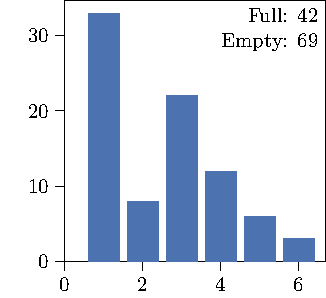
\includegraphics[width=\mymultiinner]{figures/new/abs_common-diabetes-qlibra-permutation}
      % }
    \end{subfigure}
    \begin{subfigure}{\mymultiouter}
      % \frame{
        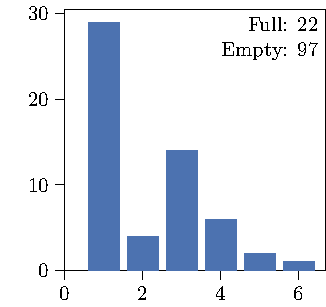
\includegraphics[width=\mymultiinner]{figures/new/abs_common-diabetes-qlibra-retraining}
      % }
    \end{subfigure}
    \begin{subfigure}{\mymultiouter}
      % \frame{
        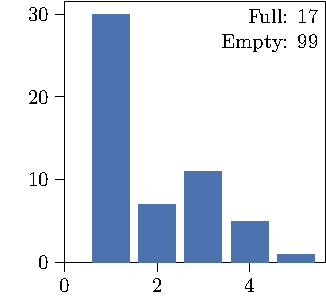
\includegraphics[width=\mymultiinner]{figures/new/abs_common-diabetes-permutation-retraining}
      % }
    \end{subfigure}
  \end{subfigure}
  \centering
  \begin{subfigure}{\textwidth}
    \centering
    \begin{subfigure}{\mymultiouter}
        \centering
        % \frame{
          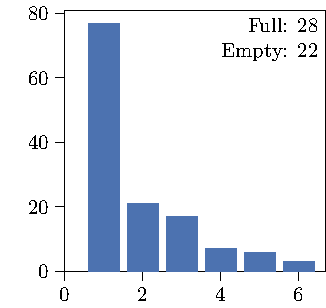
\includegraphics[width=\mymultiinner]{figures/new/relaxed_common-diabetes-qlibra-permutation}
        % }
    \end{subfigure}
    \begin{subfigure}{\mymultiouter}
        \centering
        % \frame{
          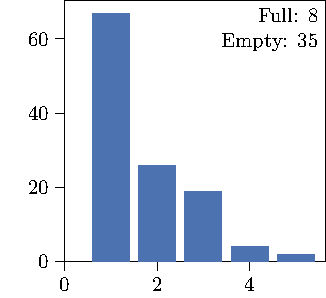
\includegraphics[width=\mymultiinner]{figures/new/relaxed_common-diabetes-qlibra-retraining}
        % }
    \end{subfigure}
    \begin{subfigure}{\mymultiouter}
        \centering
        % \frame{
          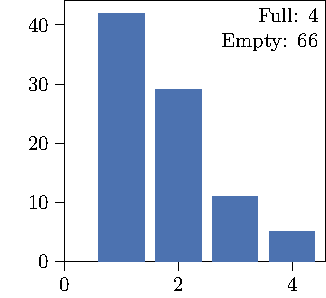
\includegraphics[width=\mymultiinner]{figures/new/relaxed_common-diabetes-permutation-retraining}
        % }
    \end{subfigure}
  \end{subfigure}
  \centering
  \begin{subfigure}{\textwidth}
    \centering
    \begin{subfigure}{\mymultiouter}
        \centering
        % \frame{
          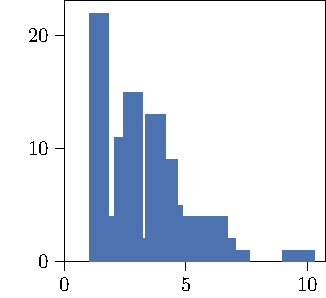
\includegraphics[width=\mymultiinner]{figures/new/eucledian-diabetes-qlibra-permutation}
        % }
    \end{subfigure}
    \begin{subfigure}{\mymultiouter}
        \centering
        % \frame{
          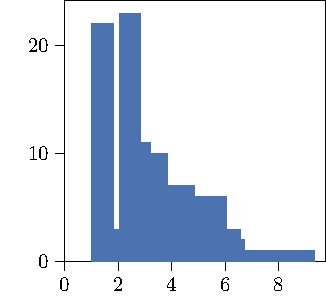
\includegraphics[width=\mymultiinner]{figures/new/eucledian-diabetes-qlibra-retraining}
        % }
    \end{subfigure}
    \begin{subfigure}{\mymultiouter}
        \centering
        % \frame{
          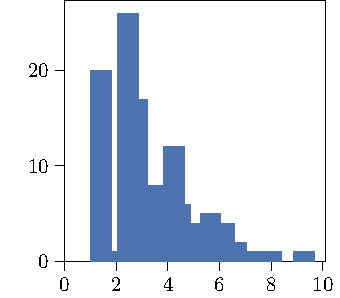
\includegraphics[width=\mymultiinner+4pt]{figures/new/eucledian-diabetes-permutation-retraining}
        % }
      \end{subfigure}
  \end{subfigure}
  \centering
  \begin{subfigure}{\textwidth}
    \centering
    \begin{subfigure}{\mymultiouter}
        \centering
        % \frame{
          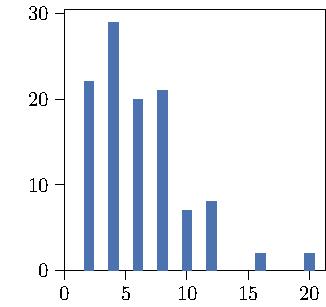
\includegraphics[width=\mymultiinner]{figures/new/manhattan-diabetes-qlibra-permutation}
        % }
    \end{subfigure}
    \begin{subfigure}{\mymultiouter}
        \centering
        % \frame{
          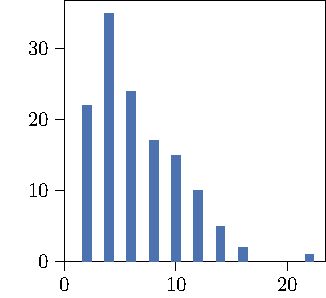
\includegraphics[width=\mymultiinner]{figures/new/manhattan-diabetes-qlibra-retraining}
        % }
    \end{subfigure}
    \begin{subfigure}{\mymultiouter}
        \centering
        % \frame{
          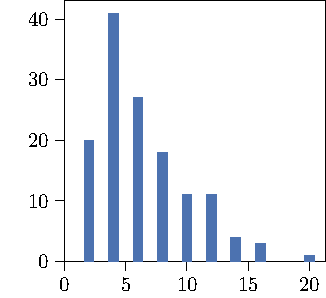
\includegraphics[width=\mymultiinner]{figures/new/manhattan-diabetes-permutation-retraining}
        % }
      \end{subfigure}
  \end{subfigure}
    \caption{Experimental overview regarding the \diabetes{} dataset.}
    \labfig{diabetes}
\end{figure}


% \begin{figure}[p]
%     \centering
%     % First row
%     \begin{tabular}{c c c c}
%         \parbox[m]{1em}{\centering \rotatebox{90}{Label 1}}
%           & 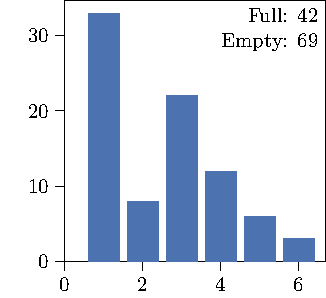
\includegraphics[width=0.3\textwidth]{figures/new/abs_common-diabetes-qlibra-permutation}
%           & 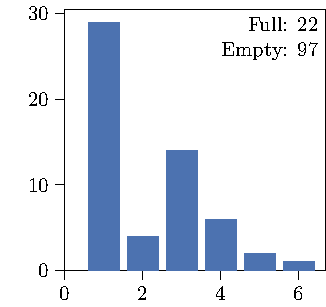
\includegraphics[width=0.3\textwidth]{figures/new/abs_common-diabetes-qlibra-retraining}
%           & 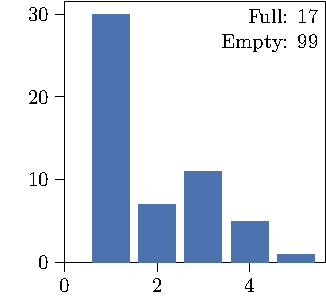
\includegraphics[width=0.3\textwidth]{figures/new/abs_common-diabetes-permutation-retraining} \\
%         \parbox[c]{1em}{\centering \rotatebox{90}{Label 1}}
%           & 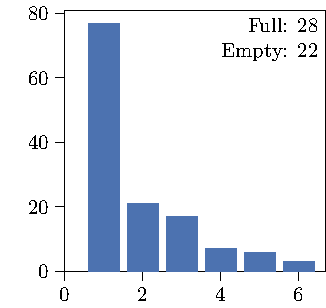
\includegraphics[width=0.3\textwidth]{figures/new/relaxed_common-diabetes-qlibra-permutation}
%           & 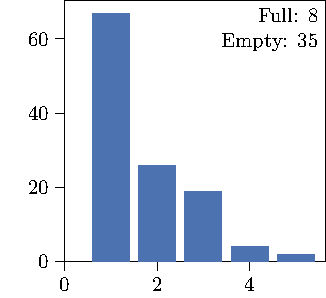
\includegraphics[width=0.3\textwidth]{figures/new/relaxed_common-diabetes-qlibra-retraining}
%           & 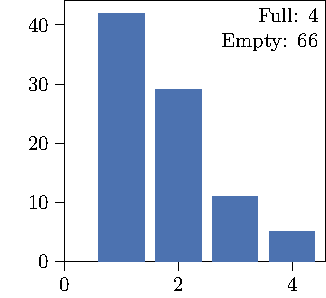
\includegraphics[width=0.3\textwidth]{figures/new/relaxed_common-diabetes-permutation-retraining} \\
%         \parbox[c]{1em}{\centering \rotatebox{90}{Label 1}}
%           & 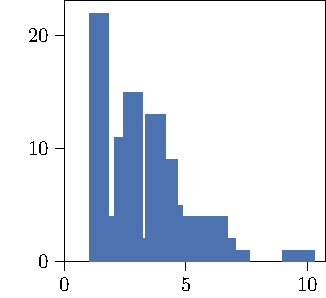
\includegraphics[width=0.3\textwidth]{figures/new/eucledian-diabetes-qlibra-permutation}
%           & 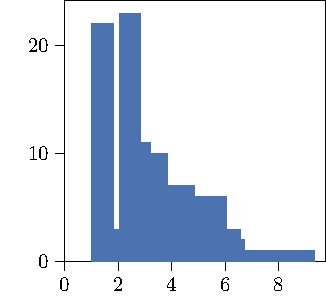
\includegraphics[width=0.3\textwidth]{figures/new/eucledian-diabetes-qlibra-retraining}
%           & 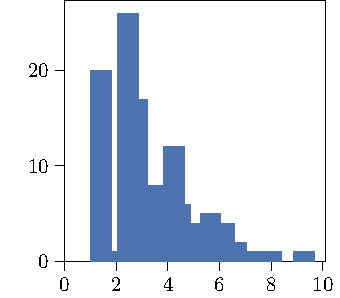
\includegraphics[width=0.3\textwidth]{figures/new/eucledian-diabetes-permutation-retraining} \\
%         \parbox[c]{1em}{\centering \rotatebox{90}{Label 1}}
%           & 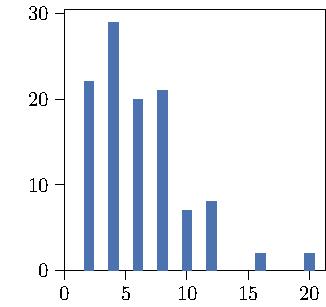
\includegraphics[width=0.3\textwidth]{figures/new/manhattan-diabetes-qlibra-permutation}
%           & 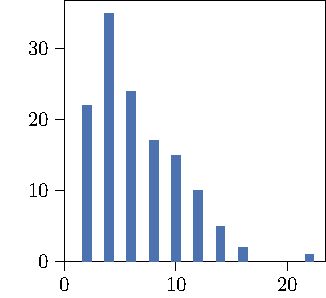
\includegraphics[width=0.3\textwidth]{figures/new/manhattan-diabetes-qlibra-retraining}
%           & 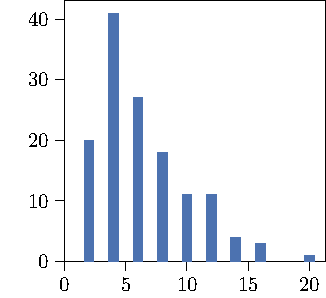
\includegraphics[width=0.3\textwidth]{figures/new/manhattan-diabetes-permutation-retraining} \\
%         & Label A & Label B & Label C \\
%     \end{tabular}
%     \caption{Your overall caption here.}
% \end{figure}






\begin{figure}[p]
  \centering
  \begin{subfigure}{\textwidth}
    \centering
    \begin{subfigure}{\mymultiouter}
      % \frame{
        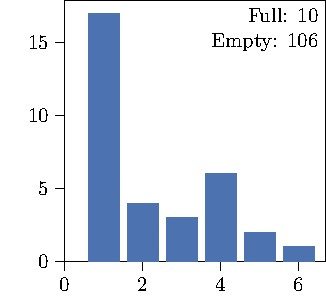
\includegraphics[width=\mymultiinner]{figures/new/abs_common-wine-qlibra-permutation}
      % }
    \end{subfigure}
    \begin{subfigure}{\mymultiouter}
      % \frame{
        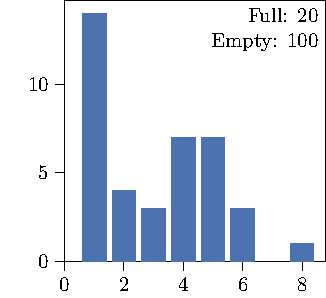
\includegraphics[width=\mymultiinner]{figures/new/abs_common-wine-qlibra-retraining}
      % }
    \end{subfigure}
    \begin{subfigure}{\mymultiouter}
      % \frame{
        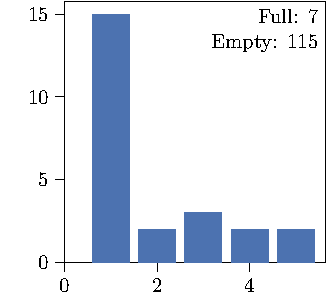
\includegraphics[width=\mymultiinner]{figures/new/abs_common-wine-permutation-retraining}
      % }
    \end{subfigure}
  \end{subfigure}
  \centering
  \begin{subfigure}{\textwidth}
    \centering
    \begin{subfigure}{\mymultiouter}
        \centering
        % \frame{
          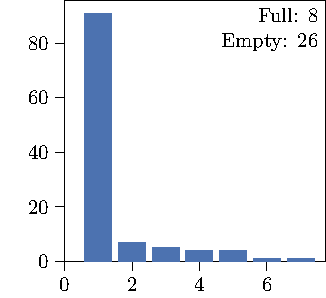
\includegraphics[width=\mymultiinner]{figures/new/relaxed_common-wine-qlibra-permutation}
        % }
    \end{subfigure}
    \begin{subfigure}{\mymultiouter}
        \centering
        % \frame{
          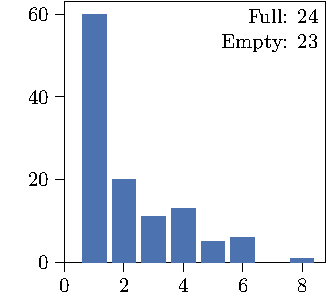
\includegraphics[width=\mymultiinner]{figures/new/relaxed_common-wine-qlibra-retraining}
        % }
    \end{subfigure}
    \begin{subfigure}{\mymultiouter}
        \centering
        % \frame{
          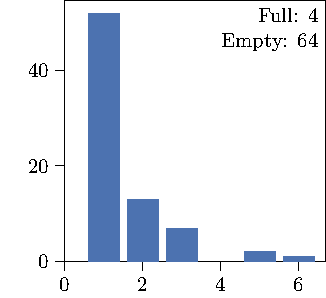
\includegraphics[width=\mymultiinner]{figures/new/relaxed_common-wine-permutation-retraining}
        % }
    \end{subfigure}
  \end{subfigure}
  \centering
  \begin{subfigure}{\textwidth}
    \centering
    \begin{subfigure}{\mymultiouter}
        \centering
        % \frame{
          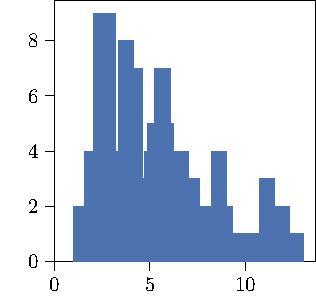
\includegraphics[width=\mymultiinner]{figures/new/eucledian-wine-qlibra-permutation}
        % }
    \end{subfigure}
    \begin{subfigure}{\mymultiouter}
        \centering
        % \frame{
          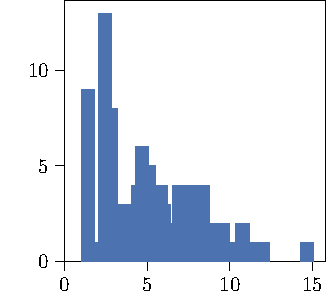
\includegraphics[width=\mymultiinner]{figures/new/eucledian-wine-qlibra-retraining}
        % }
    \end{subfigure}
    \begin{subfigure}{\mymultiouter}
        \centering
        % \frame{
          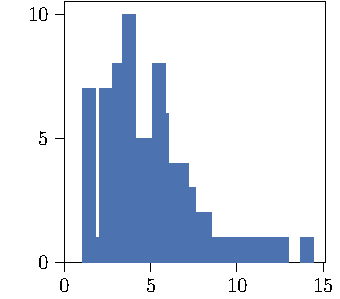
\includegraphics[width=\mymultiinner]{figures/new/eucledian-wine-permutation-retraining}
        % }
      \end{subfigure}
  \end{subfigure}
  \centering
  \begin{subfigure}{\textwidth}
    \centering
    \begin{subfigure}{\mymultiouter}
        \centering
        % \frame{
          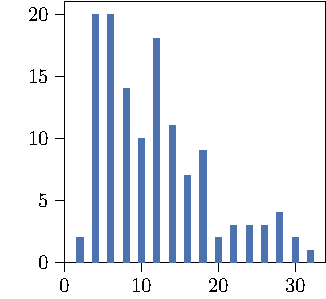
\includegraphics[width=\mymultiinner]{figures/new/manhattan-wine-qlibra-permutation}
        % }
    \end{subfigure}
    \begin{subfigure}{\mymultiouter}
        \centering
        % \frame{
          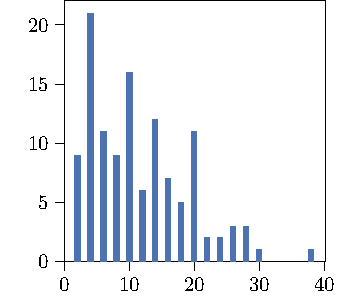
\includegraphics[width=\mymultiinner]{figures/new/manhattan-wine-qlibra-retraining}
        % }
    \end{subfigure}
    \begin{subfigure}{\mymultiouter}
        \centering
        % \frame{
          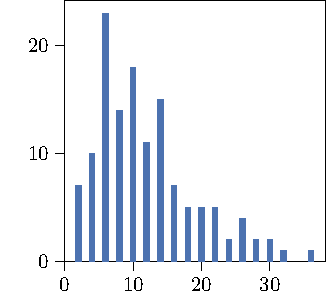
\includegraphics[width=\mymultiinner]{figures/new/manhattan-wine-permutation-retraining}
        % }
      \end{subfigure}
  \end{subfigure}
    \caption{Experimental overview regarding the ``\wine{}'' dataset.}
    \labfig{wine}
\end{figure}



\begin{figure}[p]
  \centering
  \begin{subfigure}{\textwidth}
    \centering
    \begin{subfigure}{\mymultiouter}
      % \frame{
        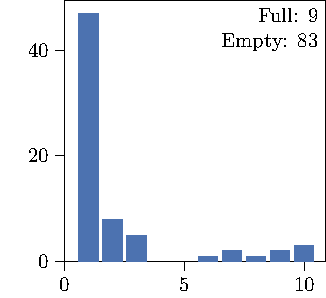
\includegraphics[width=\mymultiinner]{figures/new/abs_common-rain_sydney-qlibra-permutation}
      % }
    \end{subfigure}
    \begin{subfigure}{\mymultiouter}
      % \frame{
        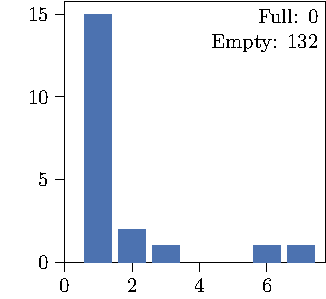
\includegraphics[width=\mymultiinner]{figures/new/abs_common-rain_sydney-qlibra-retraining}
      % }
    \end{subfigure}
    \begin{subfigure}{\mymultiouter}
      % \frame{
        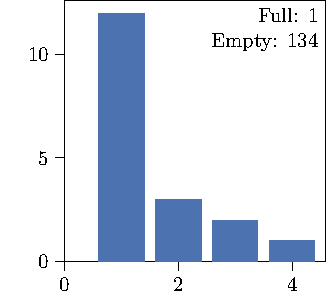
\includegraphics[width=\mymultiinner]{figures/new/abs_common-rain_sydney-permutation-retraining}
      % }
    \end{subfigure}
  \end{subfigure}
  \centering
  \begin{subfigure}{\textwidth}
    \centering
    \begin{subfigure}{\mymultiouter}
        \centering
        % \frame{
          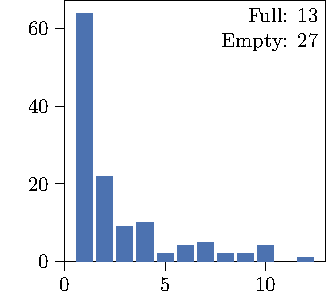
\includegraphics[width=\mymultiinner]{figures/new/relaxed_common-rain_sydney-qlibra-permutation}
        % }
    \end{subfigure}
    \begin{subfigure}{\mymultiouter}
        \centering
        % \frame{
          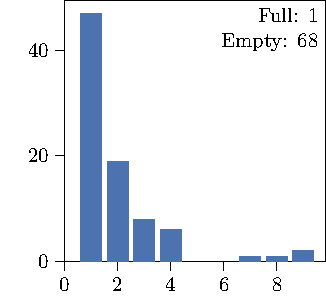
\includegraphics[width=\mymultiinner]{figures/new/relaxed_common-rain_sydney-qlibra-retraining}
        % }
    \end{subfigure}
    \begin{subfigure}{\mymultiouter}
        \centering
        % \frame{
          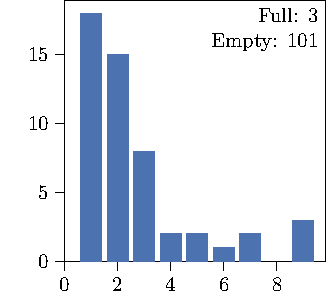
\includegraphics[width=\mymultiinner]{figures/new/relaxed_common-rain_sydney-permutation-retraining}
        % }
    \end{subfigure}
  \end{subfigure}
  \centering
  \begin{subfigure}{\textwidth}
    \centering
    \begin{subfigure}{\mymultiouter}
        \centering
        % \frame{
          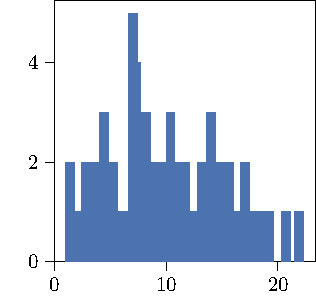
\includegraphics[width=\mymultiinner]{figures/new/eucledian-rain_sydney-qlibra-permutation}
        % }
    \end{subfigure}
    \begin{subfigure}{\mymultiouter}
        \centering
        % \frame{
          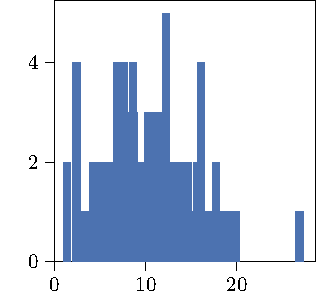
\includegraphics[width=\mymultiinner]{figures/new/eucledian-rain_sydney-qlibra-retraining}
        % }
    \end{subfigure}
    \begin{subfigure}{\mymultiouter}
        \centering
        % \frame{
          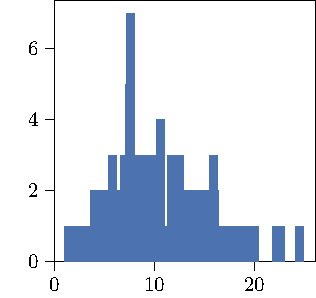
\includegraphics[width=\mymultiinner]{figures/new/eucledian-rain_sydney-permutation-retraining}
        % }
      \end{subfigure}
  \end{subfigure}
  \centering
  \begin{subfigure}{\textwidth}
    \centering
    \begin{subfigure}{\mymultiouter}
        \centering
        % \frame{
          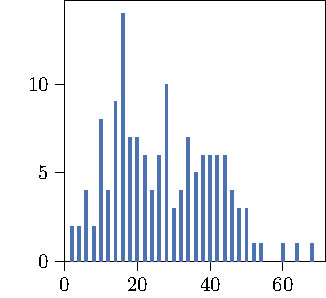
\includegraphics[width=\mymultiinner]{figures/new/manhattan-rain_sydney-qlibra-permutation}
        % }
    \end{subfigure}
    \begin{subfigure}{\mymultiouter}
        \centering
        % \frame{
          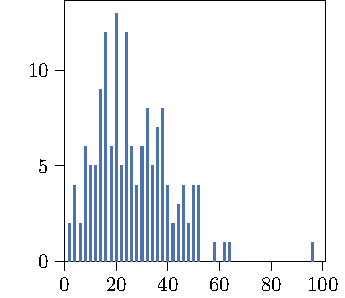
\includegraphics[width=\mymultiinner]{figures/new/manhattan-rain_sydney-qlibra-retraining}
        % }
    \end{subfigure}
    \begin{subfigure}{\mymultiouter}
        \centering
        % \frame{
          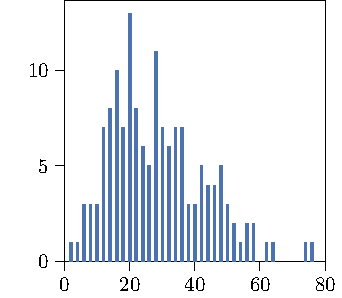
\includegraphics[width=\mymultiinner]{figures/new/manhattan-rain_sydney-permutation-retraining}
        % }
      \end{subfigure}
  \end{subfigure}
    \caption{Experimental overview regarding the ``\rain{}'' dataset.}
    \labfig{rain}
\end{figure}



\begin{figure}[p]
  \centering
  \begin{subfigure}{\textwidth}
    \centering
    \begin{subfigure}{\mymultiouter}
      % \frame{
        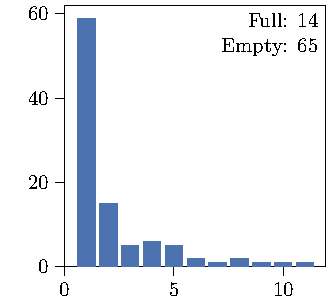
\includegraphics[width=\mymultiinner]{figures/new/abs_common-princess-qlibra-permutation}
      % }
    \end{subfigure}
    \begin{subfigure}{\mymultiouter}
      % \frame{
        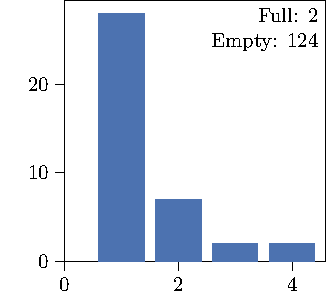
\includegraphics[width=\mymultiinner]{figures/new/abs_common-princess-qlibra-retraining}
      % }
    \end{subfigure}
    \begin{subfigure}{\mymultiouter}
      % \frame{
        \includegraphics[width=\mymultiinner]{figures/new/abs_common-princess-permutation-retraining}
      % }
    \end{subfigure}
  \end{subfigure}
  \centering
  \begin{subfigure}{\textwidth}
    \centering
    \begin{subfigure}{\mymultiouter}
        \centering
        % \frame{
          \includegraphics[width=\mymultiinner]{figures/new/relaxed_common-princess-qlibra-permutation}
        % }
    \end{subfigure}
    \begin{subfigure}{\mymultiouter}
        \centering
        % \frame{
          \includegraphics[width=\mymultiinner]{figures/new/relaxed_common-princess-qlibra-retraining}
        % }
    \end{subfigure}
    \begin{subfigure}{\mymultiouter}
        \centering
        % \frame{
          \includegraphics[width=\mymultiinner]{figures/new/relaxed_common-princess-permutation-retraining}
        % }
    \end{subfigure}
  \end{subfigure}
  \centering
  \begin{subfigure}{\textwidth}
    \centering
    \begin{subfigure}{\mymultiouter}
        \centering
        % \frame{
          \includegraphics[width=\mymultiinner]{figures/new/eucledian-princess-qlibra-permutation}
        % }
    \end{subfigure}
    \begin{subfigure}{\mymultiouter}
        \centering
        % \frame{
          \includegraphics[width=\mymultiinner]{figures/new/eucledian-princess-qlibra-retraining}
        % }
    \end{subfigure}
    \begin{subfigure}{\mymultiouter}
        \centering
        % \frame{
          \includegraphics[width=\mymultiinner]{figures/new/eucledian-princess-permutation-retraining}
        % }
      \end{subfigure}
  \end{subfigure}
  \centering
  \begin{subfigure}{\textwidth}
    \centering
    \begin{subfigure}{\mymultiouter}
        \centering
        % \frame{
          \includegraphics[width=\mymultiinner]{figures/new/manhattan-princess-qlibra-permutation}
        % }
    \end{subfigure}
    \begin{subfigure}{\mymultiouter}
        \centering
        % \frame{
          \includegraphics[width=\mymultiinner]{figures/new/manhattan-princess-qlibra-retraining}
        % }
    \end{subfigure}
    \begin{subfigure}{\mymultiouter}
        \centering
        % \frame{
          \includegraphics[width=\mymultiinner]{figures/new/manhattan-princess-permutation-retraining}
        % }
      \end{subfigure}
  \end{subfigure}
    \caption{Experimental overview regarding the ``\princess{}'' dataset.}
    \labfig{princess}
\end{figure}


\section{Evaluation of \qlibraname{}}[\qlibraname]
\labsec{eval-qlibra}

We implement \qlibraname{} in \python{} as part of the tool \libra\sidenote{\libraurl}.
%
To demonstrate its effectiveness, we evaluated it on neural networks trained on
%popular datasets in the fairness literature. Specifically, we used the Japanese Credit Screening\sidenote{\rurl{archive.ics.uci.edu/ml/datasets/Japanese+Credit+Screening}} (\textsc{japanese} in the following) and
the
Adult dataset\sidenote{\rurl{archive.ics.uci.edu/ml/datasets/adult}} from the UCI Machine Learning Repository.
%
The dataset assigns to individuals a yearly income greater or smaller than \$50k based on personal attributes such as education and occupation but also gender, marital status, or race.
The gender is set to be the sensitive input feature.
%
% We show below the experimental results on the smaller neural networks used by \sidetextcite{Urban2020}, which better demonstrate the benefits of our implementation compared to its preliminary version.
% %
% In practice, \textcite{Urban2020} have already shown that the approach can scale to much larger networks with sizes on par with the literature on fairness certification, \eg, \sidecite{Manisha2020,Yurochkin2020}.
%
The neural networks were trained with Keras for 50 iterations, using the RMSprop optimizer with the default learning rate, and categorical cross-entropy as the loss function.
%
All networks are open source as part of \libra.

%We performed all the experiments using the CLEPS infrastructure\sidenote{\rurl{paris-cluster-2019.gitlabpages.inria.fr/cleps/cleps-userguide/}}, on the \texttt{cpu\_homogen} partition. Based on a 64-core Intel\textsuperscript{\tiny{\textregistered}} Xeon\textsuperscript{\tiny{\textregistered}} 5218 CPU @ 2.4GHz machine with 192GB of RAM, running CentOS 7.7. with linux kernel 3.10.0.
%

The experiments were conducted on the Inria Paris \textsc{cleps} infrastructure\sidenote{\rurl{paris-cluster-2019.gitlabpages.inria.fr/cleps/cleps-userguide/}}, on a machine with two 16-core Intel\textsuperscript{\tiny{\textregistered}} Xeon\textsuperscript{\tiny{\textregistered}} 5218 CPU @ 2.4GHz, 192GB of RAM, and running CentOS 7.7. with linux kernel 3.10.0.
%
For each experiment, we report the average results of five executions to account for the effect of randomness of the environment.


\subsection{Effect of Neural Network Structure on Precision and Scalability.}

The precision and scalability of \libra's analysis depend on the analyzed neural network. \reftab{models} shows the result of running \libra{} on different neural networks with different choices for the abstract domain used by the pre-analysis.
Column $|\textsc{m}|$ refers to the analyzed neural network by the number of its \relu{} activations. From top to bottom, the neural networks have the following number of hidden layers and nodes per layer: $2$ and $5$, $4$ and $3$, $4$ and $5$, $4$ and $10$, and $9$ and $5$.
% \todo{larger networks are not actually needed for tabular datasets.
% These network sizes are on par with the fairness verification literature, e.g., see \sidecite{Manisha2020,Yurochkin2020}.
% However, \sidecite{Urban2020} demonstrates the approach for networks with over than $1000$ nodes.}
% Indeed, these networks sizes are on par with the fairness verification literature, e.g., see \sidecite{Manisha2020,Yurochkin2020}.
% \todo{let's be careful here; the nets in the literature are slightly larger, having hundreds of nodes; we should say it as in the rebuttal}
We configured the pre-analysis with lower bound $\lowerbound = 0.5$ and upper bound $\upperbound = 5$. Each column shows the chosen abstract domain. We show here the results for \boxes, \symbolic, \deeppoly, \neurify, and the reduced product \textsc{deeppoly+neurify+symbolic} (\ie, \reducedproduct{} in the \reftab{models}), which is the most precise of all possible reduced products.
%
% reftabs~\reftab{models1-ext} and~\reftab{models2-ext} in Appendix~\ref{apx:evaluation} show the results for all domain choices, including all possible reduced products.
%
The \textsc{input} rows show the average input-space coverage, that is, the average
%over $5$ executions)
percentage of the input space that \libra{} was able to analyze with the chosen pre-analysis configuration.
% Column $|\textsc{c}|$ shows the total number of analyzed input space partitions, while column $|\textsc{f}|$ shows the number of activation patterns (left) and feasible input partitions (right) passed to the backward analysis.
The \textsc{time} rows show the average running time.

\newcolumntype{P}[1]{>{\centering\arraybackslash}p{#1}}
\begin{table}[t]
  \caption{Comparison of the amount of fair input space discovered by different abstract domains of \libra{} on different neural networks.}
  \labtab{models}
  \centering
  \resizebox{\textwidth}{!}{%
  \begin{tabular}{ P{2em} P{5em} P{5em} P{5em} P{5em} P{5em} P{3em} }
    $|\defmodel|$ & \boxes & \symbolic & \deeppoly & \neurify &  \reducedproduct &  \\
    \toprule
    %
    \rowcolor{gray!10} \cellcolor{white} & $96.81\%$ & \textbf{98.72}$\%$ & $98.37\%$ & $98.51\%$ &  \textbf{99.44}$\%$
    %\cellcolor{seabornGreen!20}
    & \textsc{input} \\
    %
    %\cellcolor{seabornGreen!20}
    \multirow{-2}{*}{$10$}& 6m 32s & \textbf{4m 52s} & 3m 23s & 4m 27s &  \textbf{4m 40s}
    %\cellcolor{seabornGreen!20}
    &  \textsc{time} \\
    %
    \rowcolor{gray!10}
    \cellcolor{white}
    & $69.10\%$ & \textbf{76.70}$\%$ & $66.39\%$ & $64.58\%$ &  \textbf{77.29}$\%$
    %\cellcolor{seabornYellow!20}
    & \textsc{input} \\
    %
    %\cellcolor{seabornYellow!20}
    \multirow{-2}{*}{$12$}& 4m 53s & \textbf{2m 27s} & 2m 0s & 1m 31s & \textbf{2m 30s}
    %\cellcolor{seabornYellow!20}
    & \textsc{time} \\
    %
    \rowcolor{gray!10} \cellcolor{white} & $41.01\%$ & \textbf{56.11}$\%$ & $56.10\%$ & $53.06\%$ &  \textbf{68.23}$\%$%\cellcolor{seabornOrange!20}
    & \textsc{input} \\
    %
    %\cellcolor{seabornOrange!20}
    \multirow{-2}{*}{$20$}& 4m 8s & \textbf{9m 7s} & 3m 43s & 3m 53s & \textbf{8m 9s}%\cellcolor{seabornOrange!20}
    & \textsc{time} \\
    %
    \rowcolor{gray!10} \cellcolor{white} & $0.35\%$ & $34.72\%$ & \textbf{38.69$\%$} & $41.22\%$ & \textbf{51.18$\%$}%\cellcolor{seabornRed!20}
    & \textsc{input} \\
    %
    %\cellcolor{seabornRed!20}
    \multirow{-2}{*}{$40$}& 1m 3s & 7m 2s & \textbf{37m 16s} & 10m 33s & \textbf{38m 27s}
    %\cellcolor{seabornRed!20}
    & \textsc{time} \\
    %
    \rowcolor{gray!10} \cellcolor{white} & $1.74\%$ & $43.78\%$ & $51.21\%$ & $50.59\%$ & \textbf{55.53}$\%$%\cellcolor{seabornBlue!20}
    & \textsc{input} \\
    %
    %\cellcolor{seabornBlue!20}
    \multirow{-2}{*}{$45$}& 50s & 3m 42s & 5m 14s & 5m 10s & \textbf{6m 22s}
    %\cellcolor{seabornBlue!20}
    & \textsc{time} \\
    \bottomrule
    \end{tabular}
  }
\end{table}

For all neural networks, \reducedproduct{} achieves the highest input-space coverage, an improvement of up to $12.49\%$ over the best coverage obtained with only the abstract domains available in the preliminary version of \libra{} \sidecite{Urban2020} (\ie, with respect to the \deeppoly{} domain for $|\textsc{m}| = 40$). Interestingly, such an improvement comes at the cost of a very modest increase in running time (\ie, just over $1$ minute).
% More often, the running time even decreases.
Indeed, using a more precise abstract domain for the pre-analysis generally results in fewer input space partitions being passed to the backward analysis and, in turn, this reduces the overall running time.

For the smallest neural networks (\ie, $|\textsc{m}| \in \{10, 12, 20\}$), the \symbolic{} abstract domain is the second-best choice in terms of input-space coverage. This is likely due to the convex \relu{} approximations of \deeppoly{} and \neurify{} which in some case produce a negative lower bound (\cf{} \reffig{deeppoly} and \reffig{neurify}),
%in \ref{subsec:domains}),
while \symbolic{} always sets the lower bound to zero (\cf{} \reffig{naive}).
%in \ref{subsec:domains}).

Finally, for the largest neural networks (\ie, $|\textsc{m}| \in \{40, 45\}$), it is the structure of the network (rather than its number of \relu{} activations) that impacts the precision and scalability of the analysis: for the deep but narrow network (\ie, $|\textsc{m}| = 45$), \libra{} achieves a higher input-space coverage in a shorter running time than for the shallow but wide network (\ie, $|\textsc{m}| = 40$). \\
%

\subsection{Precision-vs-Scalability Tradeoff.}
The configuration of \libra{}'s pre-analysis allows trading-off between precision and scalability.
\reftab{configurations} shows the average results of running \libra{} on the neural network with $20$ \relu{}s
with different lower and upper bound configurations, and different choices for the abstract domain used by the pre-analysis.
%
Columns $\lowerbound$ and $\upperbound$ show the configured lower and upper bounds. We tried $\lowerbound \in \{0.5, 0.25\}$ and $\upperbound \in \{3, 5\}$. We again show the results for the \boxes, \symbolic, \deeppoly, \neurify{} abstract domains, and the most precise reduced product domain \textsc{deeppoly+neurify+symbolic} (\ie, \reducedproduct{} in \reftab{configurations}).
% , while \reftab{configurations-ext} in Appendix~\ref{apx:evaluation} shows the results for all domain choices.
%
%The differences between the results shown for the same neural network in \reftab{models} and \reftab{configurations} with $\lowerbound = 0.5$ and $\upperbound = 5$ are due to random choices that happen during the analysis. Indeed, to take account of this randomness, we show average results over $5$ executions. However, these differences concerning the input space coverage are always within a range of $\pm 0.05\%$ (maximum difference obtained with \deeppoly).
%
%As before, column \textsc{input} shows the input-space coverage, column $|\textsc{c}|$ shows the total number of analyzed input space partitions, column $|\textsc{f}|$ shows the number of activation patterns (left) and feasible input partitions (right) passed to the backward analysis. Finally, column \textsc{time} shows the running time.

\begin{table}[b]
  \caption{Comparison on how the fair input space discovered by \libra{} is affected by different lower and upper bound configurations.}
  \labtab{configurations}
  \centering
  \resizebox{\textwidth}{!}{%
  \begin{tabular}{ P{2em}  P{2em}  P{5em}  P{5em}  P{5em}  P{5em} P{5em} P{3em} }
    $\lowerbound$ & $\upperbound$ & \textsc{boxes} & \textsc{symbolic} & \textsc{deeppoly} & \textsc{neurify} & \reducedproduct & \\
    \toprule
    %
    \rowcolor{gray!10} \cellcolor{white} & \cellcolor{white} & \textbf{37.88}$\%$ & $48.78\%$ & $49.01\%$ & $46.49\%$ & \textbf{59.20}$\%$
    %\cellcolor{seabornGreen!20}
    & \textsc{input} \\
    %
    \cellcolor{white} & \cellcolor{white} \multirow{-2}{*}{$3$} & 36s & 42s & 1m 35s & 32s & 1m 58s
    %\cellcolor{seabornGreen!20}
    & \textsc{time} \\
    %
    \rowcolor{gray!10} \cellcolor{white} & \cellcolor{white} & \textbf{41.01}$\%$ & $56.11\%$ & $56.15\%$ & $53.06\%$ & \textbf{68.23}$\%$
    %\cellcolor{seabornYellow!20}
    & \textsc{input} \\
    %
    \cellcolor{white} \multirow{-4}{*}{$0.5$}& \cellcolor{white} \multirow{-2}{*}{$5$} & 4m 8s & 9m 10s & 3m 47s & 3m 57s & 8m 16s
    %\cellcolor{seabornYellow!20}
    & \textsc{time} \\
    \midrule
    %
    \rowcolor{gray!10} \cellcolor{white} & \cellcolor{white} & \textbf{70.62}$\%$ & $83.63\%$ & $81.82\%$ & $81.40\%$ & \textbf{87.04}$\%$
    %\cellcolor{seabornOrange!20}
    & \textsc{input} \\
    %
    \cellcolor{white} & \cellcolor{white} \multirow{-2}{*}{$3$} & 5m 49s & 5m 55s & 5m 20s & 5m 20s &7m 12s
    %\cellcolor{seabornOrange!20}
    & \textsc{time} \\
    %
    \rowcolor{gray!10} \cellcolor{white} & \cellcolor{white} & \textbf{83.06}$\%$ & $91.67\%$ & $91.58\%$ & $92.33\%$ & \textbf{95.48}$\%$
    %\cellcolor{seabornRed!20}
    & \textsc{input} \\
    %
    \cellcolor{white} \multirow{-4}{*}{$0.25$}& \cellcolor{white} \multirow{-2}{*}{$5$} & 26m 43s & 21m 8s & 22m 8s & 25m 54s & 21m 58s
    %\cellcolor{seabornRed!20}
    & \textsc{time} \\
    \bottomrule
    \end{tabular}
}
\end{table}

As expected, decreasing the lower bound $\lowerbound$ or increasing the upper bound $\upperbound$ improves the input-space coverage (\textsc{input} rows) and increases the running time (\textsc{time} rows). We obtain an improvement of up to $12.44\%$ by increasing $\upperbound$ from $3$ to $5$ (with $\lowerbound = 0.25$ and $\boxes$), and up to $42.05\%$ by decreasing $\lowerbound$ from $0.5$ to $0.25$ (with $\upperbound = 5$ and $\boxes$). The smaller is $\lowerbound$ and the larger is $\upperbound$, the higher is the impact on the running time. Once again, for all lower and upper bound configurations, \textsc{deeppoly+neurify+symbolic} achieves the highest input-space coverage, improving up to $12.08\%$ with respect to \deeppoly{} with $\lowerbound = 0.5$ and $\upperbound = 5$. The improvement is more important for configurations with larger lower bounds.

Notably, \reftab{configurations} shows that \emph{none among the \symbolic, \deeppoly, and \neurify{} abstract domains is always more precise than the others}. There are cases where even \symbolic{} (implemented by \sidecite{Wang2018b}) outperforms \neurify{} (implemented by \sidecite{Wang2018a} which is the successor of \cite{Wang2018b} and is believed to be strictly superior to its predecessor), e.g., configuration $\lowerbound=0.5$ and $\upperbound=5$. We thus argue
for using reduced products of abstract domains also in other contexts beyond fairness certification, e.g., verifying local robustness~\sidecite{Li2019,Singh2019} or verifying functional properties of neural networks~\sidecite{Katz2017}.



\subsection{Leveraging Multiple CPUs.}
The optimal pre-analysis configuration in terms of precision or scalability depends on the analyzed neural network.
%
In order to push \libra{} to its limits and obtain $100\%$ input-space coverage on the neural network with 20 \relu{}s, we used the configuration auto-tuning mechanism starting with $\lowerbound = 1$ and $\upperbound = 0$ (\ie, the most restrictive lower and upper bound configuration) and setting $\minlowerbound = 0$ and $\maxupperbound = 20$ (\ie, the most permissive configuration).
% (in practice, analyzing the entire input space is not necessarily needed).
For all choices of abstract domains, the pre-analysis eventually stabilizes with lower bound $\lowerbound = 0.015625$ and upper bound $\upperbound = 6$.

\pgfplotstableread[row sep=\\,col sep=&]{
    cpu & boxes & symbolic & deeppoly & neurify & deeppoly+ neurify+ symbolic \\
    4 & 19.33 & 7.65 & 7.91 & 8.33 & 6.72\\
    8 & 10.62 & 4.22 & 4.27 & 4.4 & 3.58\\
    16 & 6.06 & 2.34 & 2.46 & 2.5 & 2.07\\
    32 & 4.09 & 1.55 & 1.63 & 1.66 & 1.32\\
    64 & 3.62 & 1.48 & 1.49 & 1.52 & 1.21\\
    }\datapercpu

\begin{figure}[t]
  \centering
  \begin{tikzpicture}
  \begin{axis}[
      % title={Comparison of Running Times for Different Number of CPUs},
      xlabel={Number of CPUs},
      ymax=12,ymin=0,
      ylabel={Average Running Time [hours]},
      symbolic x coords={4,8,16,32,64},
      xtick distance=1,
      % legend columns=2,
      % legend style={
      %     name=legenda,
      %     draw=none,
      %     at={(0.5,-0.2)},
      %     anchor=north
      %     },
  ]

  \addplot[color=seabornGreen!20,mark=pentagon*, mark options={fill=seabornGreen!20,draw=seabornGreen}] table[x=cpu,y=boxes]{\datapercpu};
  \addplot[color=seabornYellow!20,mark=square*, mark options={fill=seabornYellow!20,draw=seabornYellow}] table[x=cpu,y=symbolic]{\datapercpu};

  \addplot[color=seabornOrange!20,mark=triangle*, mark options={fill=seabornOrange!20,draw=seabornOrange}] table[x=cpu,y=deeppoly]{\datapercpu};
  \addplot[color=seabornRed!20,mark=*, mark options={fill=seabornRed!20,draw=seabornRed}] table[x=cpu,y=neurify]{\datapercpu};

  \addplot[color=seabornBlue!20,mark=diamond*, mark options={fill=seabornBlue!20,draw=seabornBlue}] table[x=cpu,y=deeppoly+ neurify+ symbolic]{\datapercpu};

  \addlegendentry{\textsc{boxes}}
  \addlegendentry{\textsc{symbolic}}
  \addlegendentry{\textsc{deeppoly}}
  \addlegendentry{\textsc{neurify}}
  \addlegendentry{\reducedproduct}
  \end{axis}

  % \begin{axis}[
  %     hide axis,
  %     ymax=25,ymin=0,
  %     symbolic x coords={4,8,16,32,64},
  %     legend columns=-1,
  %     legend style={
  %         name=legendb,
  %         draw=none,
  %         at={(0.5,-0.325)},
  %         anchor=north
  %         },
  %     ]

  % \addplot[color=seabornBlue!20,mark=diamond*, mark options={fill=seabornBlue!20,draw=seabornBlue}] table[x=cpu,y=deeppoly+ neurify+ symbolic]{\datapercpu};

  % \addlegendentry{\textsc{deeppoly+neurify+symbolic}}

  % \end{axis}
  % \node [fit=(legenda)(legendb),draw] {};
  \end{tikzpicture}
  \caption{Comparison of running times for different number of CPUs.}
  \labfig{cpus}
  \end{figure}

\reffig{cpus} compares the average running times for \boxes, \symbolic, \deeppoly, \neurify, and the reduced product \textsc{deeppoly+neurify+symbolic} (\ie, \reducedproduct) as a function of the number of available CPUs.
%
%
With \reducedproduct{} we obtained a running time improvement of $14.39\%$ over \symbolic, \ie, the fastest domain available in the preliminary version of \libra{} (a minimum improvement of $11.54\%$ with $16$ CPUs, and a maximum improvement of $18.24\%$ with $64$ vCPUs).
%
As expected, adding more CPUs always improves \libra{} running time. The most limited improvement in running time that occurs between $32$ CPUs and $64$ vCPUs is likely due to the use of hyperthreading as context switches between processes running intense numeric computations produce more overhead.
%

\begin{table}[t]
  \caption{Comparison of how the number of available affects the performance of \libra.}
  \labtab{cpus}
  \centering
  \resizebox{\textwidth}{!}{%
  \begin{tabular}{ P{3em}  P{6em}  P{6em}  P{6em}  P{6em} P{6em} P{2.4em} }
    $|\textsc{cpu}|$ & \boxes & \symbolic & \deeppoly & \neurify & \reducedproduct & \\
    \toprule
    %
    \rowcolor{gray!10} \cellcolor{white} & $100\%$ & $100\%$ & $100\%$ & $100\%$ & $100\%$%\cellcolor{mygreen!20}
    & \textsc{input} \\
    %
    %\cellcolor{mygreen!20}
    & $4.55\%$ & $5.23\%$ & $5.20\%$ & $5.11\%$ & $5.42\%$
    %\cellcolor{mygreen!20}
    & \textsc{bias} \\
    %
    \rowcolor{gray!10} \cellcolor{white} \multirow{-3}{*}{$4$} & 19h 20m 0s & 7h 38m 43s & 7h 54m 35s & 8h 19m 36s & 6h 43m 28s
    %\cellcolor{mygreen!20}
    & \textsc{time} \\
    \midrule
    %
    %\cellcolor{myyellow!20}
    & $100\%$ & $100\%$ & $100\%$ & $100\%$ & $100\%$
    %\cellcolor{myyellow!20}
     & \textsc{input} \\
    %
    \rowcolor{gray!10} \cellcolor{white} & $4.41\%$ & $5.16\%$ & $5.12\%$ & $5.18\%$ & $5.46\%$
    %\cellcolor{myyellow!20}
    & \textsc{bias} \\
    %
    %\cellcolor{myyellow!20}
    \multirow{-3}{*}{$8$} & 10h 37m 28s & 4h 13m 27s & 4h 16m 13s & 4h 24m 13s & 3h 34m 38s
    %\cellcolor{myyellow!20}
    & \textsc{time} \\
    \midrule
    %
    \rowcolor{gray!10} \cellcolor{white} & $100\%$ & $100\%$ & $100\%$ & $100\%$ & $100\%$
    %\cellcolor{myorange!20}
    & \textsc{input} \\
    %
    %\cellcolor{myorange!20}
    & $4.56\%$ & $5.19\%$ & $5.12\%$ & $5.20\%$ & $5.34\%$
    %\cellcolor{myorange!20}
    & \textsc{bias} \\
    %
    \rowcolor{gray!10}
    \cellcolor{white}
    \multirow{-3}{*}{$16$} & 6h 3m 23s & \textbf{2h 20m 37s} & 2h 27m 31s & 2h 30m 4s & \textbf{2h 4m 9s}
    %\cellcolor{myorange!20}
    & \textsc{time} \\
    \midrule
    %
    %\cellcolor{myred!20}
    & $100\%$ & $100\%$ & $100\%$ & $100\%$ & $100\%$
    %\cellcolor{myred!20}
    & \textsc{input} \\
    %
    \rowcolor{gray!10} \cellcolor{white} & $4.50\%$ & $5.11\%$ & $5.10\%$ & $5.10\%$ & $5.37\%$
    %\cellcolor{myred!20}
    & \textsc{bias} \\
    %
    %\cellcolor{myred!20}
    \multirow{-3}{*}{$32$} & 4h 5m 16s & 1h 33m 16s & 1h 37m 40s & 1h 39m 19s & 1h 19m 23s
    %\cellcolor{myred!20}
    & \textsc{time} \\
    \midrule
    %
    \rowcolor{gray!10} \cellcolor{white} & $100\%$ & $100\%$ & $100\%$ & $100\%$ & $100\%$
    %\cellcolor{mypurple!20}
    & \textsc{input} \\
    %
    %\cellcolor{mypurple!20}
    & $4.51\%$ & $5.11\%$ & $5.20\%$ & $5.16\%$ & $5.37\%$
    %\cellcolor{mypurple!20}
    & \textsc{bias} \\
    %
    \rowcolor{gray!10} \cellcolor{white} \multirow{-3}{*}{$64$} & 3h 37m 9s & \textbf{1h 28m 38s} & 1h 29m 26s & 1h 31m 28s & \textbf{1h 12m 21s}
    %\cellcolor{mypurple!20}
    & \textsc{time} \\
    \bottomrule
    \end{tabular}
}
\end{table}

\reftab{cpus} additionally shows the estimated percentage of bias detected with each abstract domain, \ie, \libra{} is able to certify fairness for about $95\%$ of the neural network input space. Note that, the bias estimate depends on the partitioning of the input space computed by the pre-analysis, \cf{} \refsec{parallel-implementation-qlibra}. This explains the different percentages found even by runs with the same abstract domain. Within the same column, the difference is at most $0.14\%$ on average.



Finally, we remark that \emph{the auto-tuning mechanisms is essential for scalability}. We tried repeating this experiment by directly
running \libra{} with the configuration at which auto-tuning stabilizes, \ie, $\lowerbound = 0.015625$ and $\upperbound = 6$. After six days it still had not completed and we had to interrupt it.

% \begin{marginfigure}
%   \centering
%   \begin{minipage}{0.45\textwidth}
%       \centering
%       \includegraphics[width=0.8\textwidth]{figures/old}
%       \caption{Former Task Scheduling}\labfig{old}
%   \end{minipage}
%   \begin{minipage}{0.45\textwidth}
%       \centering
%       \includegraphics[width=0.8\textwidth]{figures/new}
%       \caption{Current Task Scheduling}\labfig{new}
%   \end{minipage}
%   % }
% \end{marginfigure}


\begin{marginfigure}[*-7.5]
  \centering
  \includegraphics[width=\textwidth]{figures/old}
  \caption{Former Task Scheduling}
  \labfig{old}
\end{marginfigure}

\begin{marginfigure}[*13]
  \centering
  \includegraphics[width=\textwidth]{figures/new}
  \caption{Current Task Scheduling}
  \labfig{new}
\end{marginfigure}


Note that, while implementing our quantitative extension to \libra, we also improved greatly the parallelization of the tool.
In the original version of \libra{} (originally presented in \sidecite[*-12]{Urban2020}, without our quantitative extension), feasible partitions are first grouped by activation pattern, \ie, activation patterns that fix more \relu s are merged with those that fix fewer \relu s.
This way, in principle, the amount of work that the backward analysis has to do is reduced: it only needs to run once for each activation pattern, and can then perform all the checks for bias on each feasible partition. In practice, the abstract domains used in the original implementation prevented the parallelization of all bias checks, which were thus run sequentially. This prevented \libra{} from exploiting multi-core architectures effectively. %\\
% (cf. the task schedules shown in Figure~\ref{fig:old} and Figure~\ref{fig:new} in Appendix~\ref{apx:optimization}).\\
%
After our extension, we optimize the backward analysis in order to possibly repeat the analysis for the same activation pattern but allowing it to parallelize the bias checks.
\reffig{old} and \reffig{new} compare the previous and current backward analysis task scheduling on the same analysis instance. Each row in the Gantt diagrams shows computations of the same thread. Blue bars stand for activation pattern computations, while red bars indicate bias check computations, these two bars alternate throughout the whole backward computation for each processor (if possible).
As shown in \reffig{old}, the running time was determined almost completely by the task with the most associated bias checks, leaving all the other threads idle from the very beginning. The diagram in \reffig{new} is more compact, meaning that threads are always running jobs uniformly. Consequently, the backward analysis running time decreases from about $22$ to only $5$ minutes.



\section{Summary}

This chapter, presenting the evaluation of our quantitative framework on neural networks, concludes part of quantitative verification for extensional properties.
We have shown a quantitative framework to quantify the impact of input variables on the output of a program and applied it to the context of neural networks.
In the next part, we will study how to extend this framework to intensional properties, which are properties that depend on the internal state of the program.
We will quantify the impact of input variables on the number of iterations of a program.


\frenchdiv

\emph{Ce chapitre, qui présente l'évaluation de notre cadre quantitatif sur les réseaux neuronaux, conclut la partie dédiée à la vérification quantitative des propriétés extensionnelles. Nous avons montré un cadre quantitatif permettant de mesurer l'impact des variables d'entrée sur le résultat d'un programme et l'avons appliqué au contexte des réseaux neuronaux. Dans la prochaine partie, nous étudierons comment étendre ce cadre aux propriétés intentionnelles, qui sont des propriétés dépendant de l'état interne du programme. Nous quantifierons l'impact des variables d'entrée sur le nombre d'itérations d'un programme.}
